\documentclass{beamer}
\usetheme{Warsaw}
\usecolortheme{beaver}
\begin{document}

\title{Hadoop MapReduce Input Format}
\author[FAN Kai, PKU CNDS, fankai@net.pku.edu.cn]{FAN Kai}
\institute{Computer Networks and Distritued Systems Laboratory\\Peking University}
\date{2009.05.22}

\begin{frame}[label=titlepage]
    \titlepage
\end{frame}

\begin{frame}{FAQ - Hadoop Wiki}
    \alert{22. Does HDFS make block boundaries between records?} 
    \begin{itemize}
    \item No, HDFS does not provide record-oriented API and therefore is not aware of records and boundaries between them. 
    \end{itemize}
\end{frame}

\begin{frame}{Outline}
    \begin{itemize}
    \item InputSplit
        \begin{itemize}
        \item FileSplit ...
        \end{itemize}
    \item RecordReader
        \begin{itemize}
        \item LineRecordReader, KeyValueLineRecordReader, ...
        \end{itemize}
    \item InputFormat
        \begin{itemize}
        \item FileInputFormat
            \begin{itemize}
            \item TextInputFormat, KeyValueTextInputFormat, ...
            \end{itemize}
        \end{itemize}
    \end{itemize}
\end{frame}

\begin{frame}{interface org.apache.hadoop.mapred.InputSplit}
    \begin{itemize}
    \item InputSplit represents the data to be processed by an individual Mapper.
    \item Typically, it presents a byte-oriented view on the input and is the responsibility of RecordReader of the job to process this and present a record-oriented view. 
    \item Members: lenght \& locations
    \item Classes:
        \begin{itemize}
        \item \em{FileSplit}
        \item MultiFileSplit
        \item CompositeFileSplit
        \item ...
        \end{itemize}
    \end{itemize}
\end{frame}

\begin{frame}{interface org.apache.hadoop.mapred.RecordReader}
    \begin{itemize}
    \item Process record boundary and present the tasks with keys and values.
    \item \em{boolean next(K key, V value)}
    \item Classes:
        \begin{itemize}
        \item LineRecordReader
        \item KeyValueLineRecordReader
        \item SequenceFileRecordReader
        \item SequenceFileAsTextRecordReader
        \item ...
        \end{itemize}
    \end{itemize}
\end{frame}

\begin{frame}{Interface org.apache.hadoop.mapred.InputFormat}
    \begin{itemize}
    \item Tasks
        \begin{itemize}
        \item Validate the input-specification of the job.
        \item Split-up the input file(s) into logical InputSplits, each of which is then assigned to an individual Mapper.
        \item Provide the RecordReader implementation to be used to glean input records from the logical InputSplit for processing by the Mapper.
        \end{itemize}
    \item Classes
        \begin{itemize}
        \item FileInputFormat
        \item ...
        \end{itemize}
    \item RecordReader has the responsibility to respect record boundaries and present a record-view of the logical InputSplit
    \end{itemize}
\end{frame}

\begin{frame}{org.apache.hadoop.mapred.FileInputFormat}
    \begin{itemize}
    \item Split file based on size.
    \item Members:
        \begin{itemize}
        \item \em{InputSplit[] getSplits(JobConf job, int numSplits)}
        \item \em{boolean isSplitalbe(FileSystem fs, Path path)}
        \item \em{RecordReader getRecordReader()}
        \end{itemize}
    \item Classes: 
        \begin{itemize}
        \item \em{TextInputFormat}
        \item TextInputFormat
        \item KeyValueTextInputFormat
        \item SequenceFileInputFormat
        \item TeraInputFormat
        \end{itemize}
    \end{itemize}
\end{frame}

\begin{frame}{FAQ - Hadoop Wiki}
    \alert{23. How do Map/Reduce InputSplit's handle record boundaries correctly? } 
    \begin{itemize}
    \item It is the responsibility of the InputSplit's RecordReader to start and end at a record boundary. 
    \item For SequenceFile's every 2k bytes has a 20 bytes sync mark between the records.
        These sync marks allow the RecordReader to seek to the start of the InputSplit, which contains a file, offset and length and find the first sync mark after the start of the split.
        The RecordReader continues processing records until it reaches the first sync mark after the end of the split.
        The first split of each file naturally starts immediately and not after the first sync mark.
        In this way, it is guaranteed that each record will be processed by exactly one mapper. 
    \item Text files are handled similarly, using newlines instead of sync marks. 
    \end{itemize}
\end{frame}

\begin{frame}{}
    \begin{figure}
    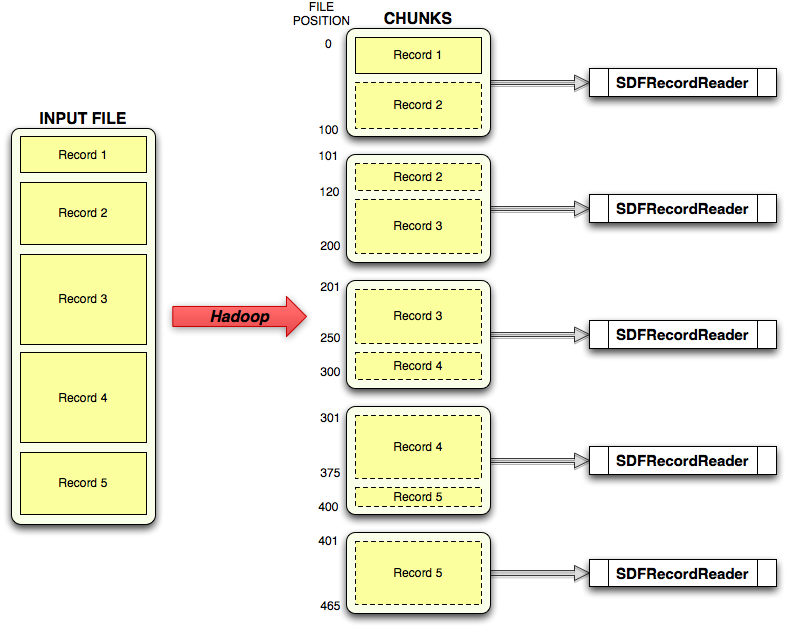
\includegraphics[width=100mm]{hadoop-chunking}
    \end{figure}
\end{frame}

\end{document}


